\documentclass[10pt,twocolumn,letterpaper]{article}

\usepackage{cvpr}
\usepackage{times}
\usepackage{epsfig}
\usepackage{graphicx}
\usepackage{amsmath}
\usepackage{amssymb}
\usepackage{float}

% Include other packages here, before hyperref.

% If you comment hyperref and then uncomment it, you should delete
% egpaper.aux before re-running latex.  (Or just hit 'q' on the first latex
% run, let it finish, and you should be clear).
\usepackage[breaklinks=true,bookmarks=false]{hyperref}

\cvprfinalcopy % *** Uncomment this line for the final submission

\def\cvprPaperID{****} % *** Enter the CVPR Paper ID here
\def\httilde{\mbox{\tt\raisebox{-.5ex}{\symbol{126}}}}

% Pages are numbered in submission mode, and unnumbered in camera-ready
%\ifcvprfinal\pagestyle{empty}\fi
\setcounter{page}{1}
\begin{document}

%%%%%%%%% TITLE
\title{Instance Segmentation for Urban Street Scenes}

\author{Francesco Bari\\
{\tt\small francesco.bari.2@studenti.unipd.it}
% For a paper whose authors are all at the same institution,
% omit the following lines up until the closing ``}''.
% Additional authors and addresses can be added with ``\and'',
% just like the second author.
% To save space, use either the email address or home page, not both
\and
Eleonora Signor\\
{\tt\small eleonora.signor@studenti.unipd.it}
}

\maketitle
%\thispagestyle{empty}

%%%%%%%%% ABSTRACT
\begin{abstract}
In questo lavoro abbiamo confrontato differenti tecniche di instance segmentation, gi\`a esistenti, sul task specifico di \textit{Urban Street Scenes}. Il nostro interesse verso il topic \`e nato dal fatto che la segmentazione delle istanze \`e uno dei compiti fondamentali della visione, tuttavia si presenta ancora complesso e non del tutto esplorato. 
%Esistono differenti approcci di instance segmentation, di seguito ne presentiamo una sottoparte, valutandone accuracy e performance su dataset multicategoriali e rivolti a quantificare la robustezza di un algoritmo.
\end{abstract}

%%%%%%%%% BODY TEXT
\section{Introduction}
La segmentazione dell'immagine \`e il processo di separazione di questa in pi\`u segmenti, in cui ciascun pixel viene associato a un tipo di oggetto. Esistono due tipologie di segmentazione dell'immagine: la segmentazione semantica e la segmentazione d'istanza. La prima contrassegna oggetti dello stesso tipo con la medesima etichetta di classe; la seconda, d'interesse del nostro lavoro, contrassegna oggetti dello stesso tipo e appartenenti a entit\`a distinte con etichette di classe differenti. L'idea che abbiamo cercato di sviluppare ha riguardato il confronto di diverse metodoligie di instance segmentation. La prima tecnica che abbiamo studiato \`e stato Mask R-CNN~\cite{Authors1_maskrcnn}, approccio a due stadi. Questa l'abbiamo scelta alla luce del riscontro positivo che ha ricevuto dal mondo della vision research, grazie al suo framework concettualmente semplice e generale, caratterizzato da un rilevamento di oggetti d'immagine efficiente, e dalla generazione in contentemporanea di una maschera di segmentazione di alta qualit\`a per ogni istanza. La tecnica che abbiamo deciso di contraporre a Mask R-CNN \`e stata BlendMask~\cite{Authors2_BlendMask}. Questa \`e invece una tecnica a uno stadio che si \`e presentata capace di superare le prestazioni di Mask R-CNN sia a livello di previsione della maschera che per tempo di formazione, su dataset MSCOCO 2017~\cite{Authors3_MSCOCO} e LVIS~\cite{Authors4_LVIS}. Ci siamo interessati a verificare se questo rimanesse valido anche su datasets, come \textit{Cityscapes}~\cite{cityscapes} e \textit{WildDash} ~\cite{wildDash}, appartenenti allo specifico topic di \textit{Urban Street Scenes}, con immagini provenienti dalle strade di tutto il mondo, con molti scenari difficili. Alcuni aspetti che abbiamo testato hanno riguardato cambiamenti di backbone, profondit\`a della rete ResNet~\cite{Authors5_ResNet} e numero di layers congelati. I risultati ottenuti ci hanno confermato quanto gi\`a annunciato dai lavori precedenti, generalizzando BlendMask come l'approccio a stadi pi\`u promettente. Al termine del nostro lavoro e per non limitare la nostra analisi abbiamo fatto qualche considerazione anche su altre tecniche di instance segmentation quali SOLOv2~\cite{Authors6_SOLOv2} e Deep Snake~\cite{Authors7_deepsnake}.

\section{Related Work}
%Le linee guida del nostro lavoro ci sono state date da differenti papers riguardanti l'instance segmentaiton task. 
%Inoltre gli abbiamo estesi con i datasets \textit{Cityscapes}~\cite{cityscapes} e \textit{WildDash} ~\cite{wildDash}.
\subsection{Stage approch} 
\textbf{Mask R-CNN}~\cite{Authors1_maskrcnn} \`e una Rete Neurale Convoluzionale che si presenta all'avanguardia in termini di segmentazione dell'immagine. \`E la variante di una Rete Neurale Profonda che rileva gli oggetti in un'immagine e vi genera una maschera di segmentazione per ciascuna istanza.
Mask R-CNN~\cite{Authors1_maskrcnn} \`e l'evoluzione successiva di Faster R-CNN~\cite{fasterRCNN}, rete neurale convoluzionale basata sulla regione, che produce per ogni oggetto candidato 3 output: l'etichetta di classe, l'offset del riquadro di delimitazione e la maschera dell'oggetto.
L'architettura della rete, Figure \ref{fig:mask_rcnn}, si compone di una CNN (backbone), che processa l'immagine e estrae la feature map. Dopodich\`e grazie alla Region Proposal Network vengono presentate le proposte o RoI, sul quale andare a fare riconosciemento del riquadro di delimitazione e previsione delle maschera (head). Inoltre prima di generare l'ouput a ciascuna RoI viene applicato RoIAlign, questo permette di ottenere una maschera dove il layout dell'oggetto viene mantenuto.

\begin{figure}[H]
\centering
  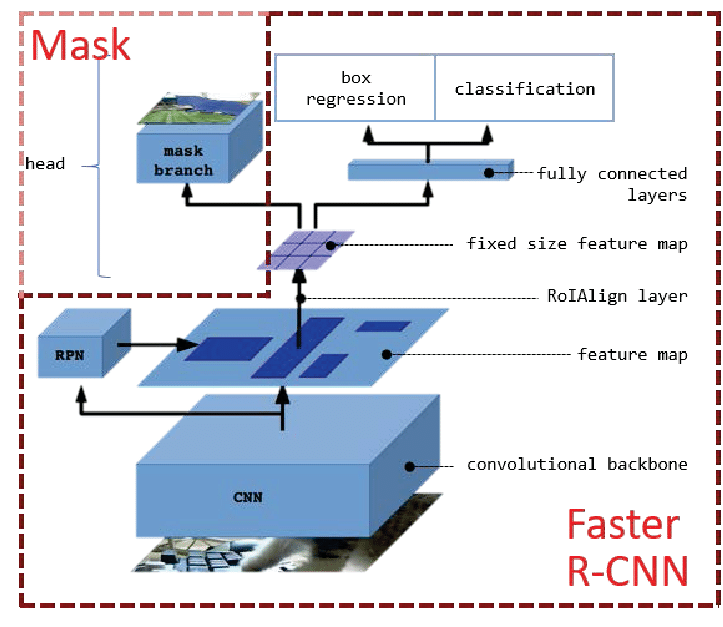
\includegraphics[width=0.7\linewidth]{./image/maskrcnn.png}
  \caption{Mask R-CNN architecture. \textit{Source: ~\cite{fig1}}}
  \label{fig:mask_rcnn}
\noindent
\end{figure}
\noindent
\indent\textbf{BlendMask}~\cite{Authors2_BlendMask} deriva dai limiti di Mask R-CNN~\cite{Authors1_maskrcnn}. Gli autori del paper definiscono come Mask R-CNN~\cite{Authors1_maskrcnn} vincoli fortemente la velocit\`a e la qualit\`a di generazione delle maschere alle heads, facendo cos\`i fatica a trattare scenari complicati e ponendo un limite alla risoluzione delle maschere. Inoltre Mask R-CNN~\cite{Authors1_maskrcnn} si presenta come un framework poco flessibile per reti multi-task. Hanno cos\`i cercato di cobinare strategie di ricerca dall'alto verso il basso e dal basso verso l'alto in FCOS~\cite{fcos}, one stage approch, che sembra in grado di superare le controparti a due stadi in termini di precisione. L'architettura di BlendMask~\cite{Authors2_BlendMask}, Figure \ref{fig:blendmask}, si compone da detector network e da una mask branch. Quest'ultima \`e partizionata in 3 parti: il modulo inferiore che si occupa di prevedere le scores map, chiamate basi; the top layer composto da un singolo strato di convoluzione e da torri, tante quante sono le input features, con il compito di predirre attention instance e un modulo blender che unisce scores con attenzioni.
\begin{figure}[H]
\centering
  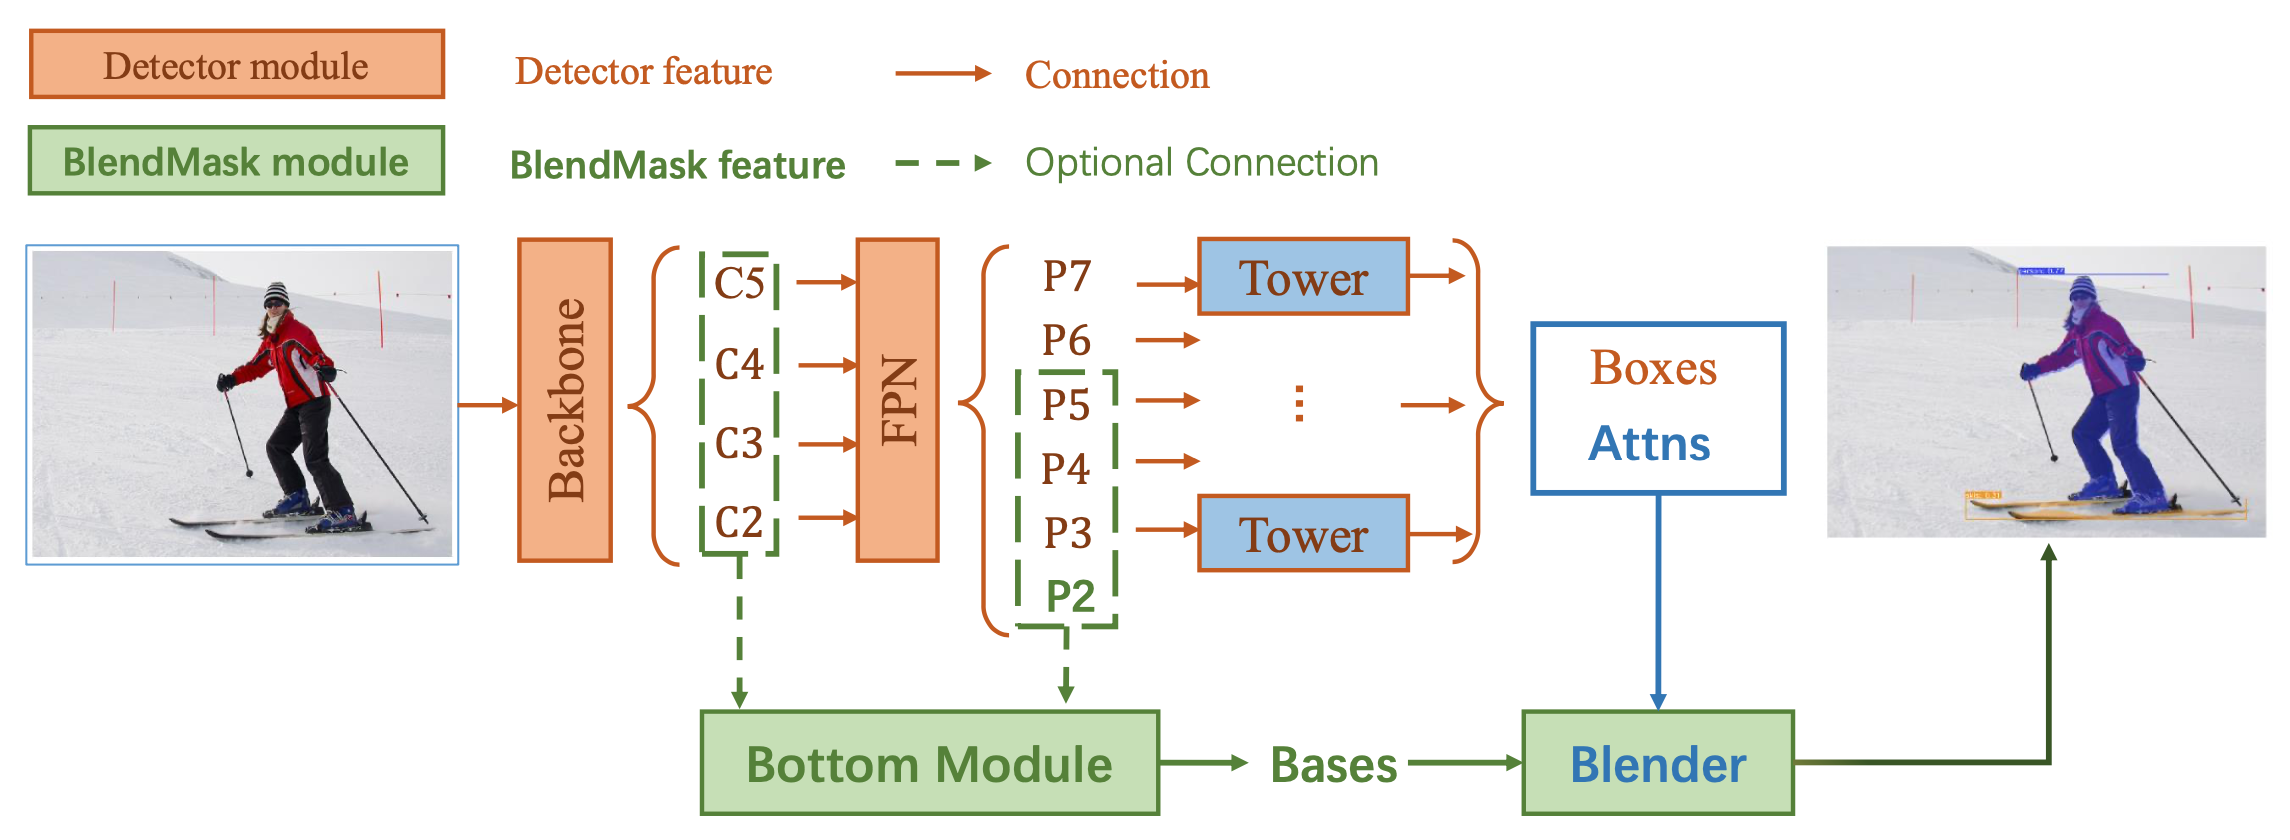
\includegraphics[width=1\linewidth]{./image/blendmask.png}
  \caption{BlendMask architecture. \textit{Source: ~\cite{Authors2_BlendMask}}}
  \label{fig:blendmask}
\noindent
\end{figure}
\noindent

\indent\textbf{SOLOv2}
\subsection{Contour-based approach}
\textbf{Deep Snake}

\section{Dataset}
Mostrare qualche immagine contenuta all'interno dei datasets. Al massimo due colonne.\\
Come sono formati (train, val, test se ci sono), le annotazioni, i json.
\subsection{Cityscapes}
Ricordarsi che ci sono categorie con frequenza diversa, sarebbe bello mettere un grafico che mostra questa quantificazione
\subsection{WildDash}
\section{Method}
Per riuscire a fare un confronto tra le diverse tecniche di instance segmentation, oggetto di questo documento, abbiamo utlizzato i seguenti approcci:
\begin{itemize}
\item proceduto con l'implentazione di modelli e successivamente fatto ricorso al metodo sperimentale per la valutazione;
\item studiato e analizzato i risultati dei papers.
\end{itemize}


\subsection{Datasets preparation}
\subsection{Training with fine-tuning}
\paragraph{Mask R-CNN}
La loss utilizzata durante il training \`e la seguente
\begin{center} min(L) $=$ min(L$_{cls}$ + L$_{box}$ + L$_{mask}$) \end{center}
L$_{cls}$ is the classification loss, L$_{box}$ is the bounding-box loss and  L$_{mask}$ is the average binary cross-entropy loss.
\paragraph{BlendMask}
La loss utilizzata durante il training \`e la seguente
\begin{center} min(L) $=$ min(semantic loss)~\cite{Authors4_semanticloss}\end{center}.

\subsection{Metrics}
\begin{itemize}
\item AP
\item numero di istanze, tempo :: accuracy visiva.confidence-threshold
\end{itemize}

\subsection{Evalutation and inference}


\section{Experiments and results}
In questa sezione descriviamo gli esperimenti che abbiamo eseguito per testare  e valutare le tecniche oggetto di questo lavoro. Tali esperimenti gli abbiamo eseguiti al termine delle fasi di studio e codifica.

\subsection{Backbone}
\label{experiments:second_trial}
La seconda serie di esperimenti, che abbiamo compiuto, riguarda la definizione della backbone. Tutte le tecniche a stadi, oggetto del confronto, sono dotate del suddetto modulo inferiore, per cui ci \`e risultato semplice uniformare le scelte architetturali in modo da poter compiere una valutazione oggettiva. Le tecniche che abbiamo confrontato sono state Mask R-CNN e BlendMask.\\
Le configurazioni constanti delle reti sono image size ...,  numero massimo di iterazioni, learning rate ..., step size a ... e fine-tuning esclusivamente agli ultimi 2 livelli.

\begin{table}[H]
\scriptsize
\begin{center}
\begin{tabular}{|c|c|c|}
\hline
Method and architecture & \textit{Cityscapes} AP & \textit{WildDash} AP\\
\hline\hline
\begin{tabular}[c]{cc}Mask R-CNN $+$ ResNet50 \\ $+$ C4 $+$ Base-RCNN-C4\end{tabular} & & \\
\hline
\begin{tabular}[c]{cc}Mask R-CNN $+$ ResNet50 \\ $+$ DC5 $+$ Base-RCNN-DilatedC5\end{tabular} & & \\
\hline
\begin{tabular}[c]{cc}Mask R-CNN $+$ ResNet50 \\ $+$ FPN $+$ Base-RCNN-FPN\end{tabular} & &\\
\hline
\end{tabular}
\end{center}
\caption{Backbone Mask R-CNN result.}
\label{mytable_backbone_MaskRCNN}
\end{table}
\noindent
Per BlendMask, oltre a settare le configurazioni costanti, avvalendoci dei risultati presentati in ... abbiamo settato R $=$ 56, M $=$ 14, K $=$ 4, sampling method for bottom bases bilinear pooling, interpolation method for top-level attentions bilinear upsampling and semantic loss. Inoltre abbiamo deciso di testare vari tipi di decoder: ProtoNet and DeepLabv3+.
\begin{table}[H]
\scriptsize
\begin{center}
\begin{tabular}{|c|c|c|}
\hline
Method and architecture & \textit{Cityscapes} AP & \textit{WildDash} AP\\
\hline\hline
\begin{tabular}[c]{cc}BlendMask with decoder ProtoNet \\ $+$ ResNet50 $+$ FPN $+$ Base-550\end{tabular} & &\\
\hline
\begin{tabular}[c]{ccc}BlendMask with decoder ProtoNet \\ $+$ ResNet50 $+$ deformable convolution \\ $+$ FPN $+$ Base-550\end{tabular} & &\\
\hline
\begin{tabular}[c]{cc}BlendMask with decoder DeepLabv3+ \\ $+$ ResNet50 $+$ FPN $+$ Base-550\end{tabular} & &\\
\hline
\begin{tabular}[c]{ccc}BlendMask with decoder DeepLabv3+ \\ $+$ ResNet50 $+$ deformable convolution \\ $+$ FPN  $+$ Base-550\end{tabular} & &\\
\hline
\end{tabular}
\end{center}
\caption{Backbone BlendMask result.}
\label{mytable_backbone_BlendMask}
\end{table}

\subsection{Deepness}
Una terza serie di esperimenti ha riguardato lo studio della profondit\`a delle reti ResNet.\\
I parametri di configurazione non definiti in modo esplicito, sono le medesime di quelle riportate nella sezione \S\ref{experiments:second_trial}.
\begin{table}[H]
\scriptsize
\begin{center}
\begin{tabular}{|c|c|c|}
\hline
Method and architecture & \textit{Cityscapes} AP & \textit{WildDash} AP\\
\hline\hline
\begin{tabular}[c]{cc}BlendMask with decoder ProtoNet \\ $+$ ResNet101 $+$ FPN $+$ Base-BlendMask\end{tabular} & &\\
\hline
\begin{tabular}[c]{ccc}BlendMask with decoder ProtoNet \\ $+$ ResNet101 $+$ deformable convolution \\$+$ FPN $+$ Base-BlendMask\end{tabular} & &\\
\hline
\end{tabular}
\end{center}
\caption{Deepness BlendMask result.}
\label{mytable_deepness_BlendMask}
\end{table}

\subsection{Freeze levels}
Per la quarta serie di esperimenti ci siamo voluti concentrare sul numero di layers da "scongelare" di ResNet durante il re-training dei pesi.\\
I parametri di configurazione non definiti in modo esplicito, sono le medesime di quelle riportate nella sezione \S \ref{experiments:second_trial}.
\begin{table}[H]
\scriptsize
\begin{center}
\begin{tabular}{|c|c|c|}
\hline
Method and architecture & \textit{Cityscapes} AP & \textit{WildDash} AP\\
\hline\hline
\begin{tabular}[c]{ccc}Mask R-CNN $+$ ResNet101 $+$ FPN \\ 1 layers freeze\end{tabular} & &\\
\hline
\begin{tabular}[c]{ccc}Mask R-CNN $+$ ResNet101 $+$ FPN \\ 3 layers freeze\end{tabular} & &\\
\hline
\begin{tabular}[c]{ccc}BlendMask with decoder ProtoNet \\ $+$ ResNet101 $+$ FPN $+$ Base-BlendMask \\ 1 layers freeze\end{tabular} & &\\
\hline
\begin{tabular}[c]{ccc}BlendMask with decoder ProtoNet \\ $+$ ResNet101 $+$ FPN $+$ Base-BlendMask \\ 3 layers freeze\end{tabular} & &\\
\hline
\end{tabular}
\end{center}
\caption{Freeze layers result.}
\label{mytable_deepness_BlendMask}
\end{table}


\subsection{Own best models}
Come ultima serie di esperimenti abbiamo cercato di individuare i modelli migliori, per ciascuna le due tecniche di instance segmentation in esame in questa sezione; tenedo conto della possibilit\`a di allenare ciascun modello solo su una singolo macchina e 1 GPU.\\
I parametri di configurazione non definiti in modo esplicito, sono le medesime di quelle riportate nella sezione \S \ref{experiments:second_trial}.

\begin{table}[H]
\scriptsize
\begin{center}
\begin{tabular}{|c|c|c|}
\hline
Dataset & method and architecture & AP\\
\hline\hline

\hline
\end{tabular}
\end{center}
\caption{Own best models result.}
\label{mytable_own_best_model}
\end{table}



\section{Conclusion}
Al massimo mezza colonna.\\
BlendMask funziona meglio di Mask RCNN, sia a livello di performance GPU che accuratezza. SOLOv2 sembra avere risultati migliori di Mask R-CNN, ma inferiori a BlendMask. Esistono anche altre tecniche che 'escono' dall'approccio a stadi, per esempio Deep Snake che pu\`o presentarsi una valida alternativa a Blender tuttavia da miglirare in futuro. Magari sarebbe possibile un'integrazione tra queste due tecniche.

\begin{thebibliography}{1}
\bibitem{Authors1_maskrcnn}
Kaiming He and Georgia Gkioxari and Piotr Dollár and Ross Girshick.
Mask R-CNN. CoRR, 2018.
\bibitem{Authors2_BlendMask}
Hao Chen, Kunyang Sun, Zhi Tian, Chunhua Shen, Yongming Huang and Youliang Yan.
BlendMask: Top-Down Meets Bottom-Up for Instance Segmentation. CoRR, 2020.
\bibitem{Authors3_MSCOCO}
Tsung-Yi Lin, Michael Maire, Serge J. Belongie, Lubomir D. Bourdev, Ross B. Girshick, James Hays, Pietro Perona, Deva Ramanan, Piotr Doll\'ar and C. Lawrence Zitnick.
Microsoft COCO: Common Objects in Context. CoRR, 2014.
\bibitem{Authors4_LVIS}
Agrim Gupta, Piotr Doll\'ar and Ross B. Girshick.
LVIS: A Dataset for Large Vocabulary Instance Segmentation. CoRR, 2019.
\bibitem{cityscapes}
Marius Cordts, Mohamed Omran, Sebastian Ramos, Timo Rehfeld, Markus Enzweiler, Rodrigo Benenson, Uwe Franke, Stefan Roth and Bernt Schiele.
The Cityscapes Dataset for Semantic Urban Scene Understanding. CoRR, 2016.
\bibitem{wildDash}
Zendel, Oliver and Honauer, Katrin and Murschitz, Markus and Steininger, Daniel and Dominguez, Gustavo Fernandez.
WildDash - Creating Hazard-Aware Benchmarks. Proceedings of the European Conference on Computer Vision, (ECCV), 2018.
\bibitem{Authors5_ResNet}
Kaiming He, Xiangyu Zhang, Shaoqing Ren and Jian Sun.
Deep Residual Learning for Image Recognition. CoRR, 2015.
\bibitem{Authors6_SOLOv2}
Xinlong Wang,Rufeng Zhang,Tao Kong, Lei Li and Chunhua Shen.
SOLOv2: Dynamic, Faster and Stronger. CoRR, 2020.
\bibitem{Authors7_deepsnake}
Sida Peng, Wen Jiang, Huaijin Pi, Hujun Bao and Xiaowei Zhou.
Deep Snake for Real-Time Instance Segmentation. CoRR, 2020.
\bibitem{fasterRCNN}
Shaoqing Ren, Kaiming He, Ross B. Girshick, Jian Sun.
Faster R-CNN: Towards Real-Time Object Detection with Region Proposal Networks. CoRR, 2015.
\bibitem{fig1}
Bienias, Lukasz \& n, Juanjo \& Nielsen, Line \& Alstrøm, Tommy. Insights Into The Behaviour Of Multi-Task Deep Neural Networks For Medical Image Segmentation. 2019.
\bibitem{fcos}
Zhi Tian, Chunhua Shen, Hao Chen and Tong He.
FCOS: Fully Convolutional One-Stage Object Detection. CoRR, 2019.
\bibitem{Authors8_semanticloss}
Xu, Jingyi and Zhang, Zilu and Friedman, Tal and Liang, Yitao and Van den Broeck, Guy.
A Semantic Loss Function for Deep Learning with Symbolic Knowledge. Proceedings of the 35th International Conference on Machine Learning, 2018.

\end{thebibliography}



\end{document}
